% Ready-to-use figure snippets for a LaTeX build run from docs/cross_power/.
% Uncomment the environments as needed.

% \begin{figure}[t]
%   \centering
%   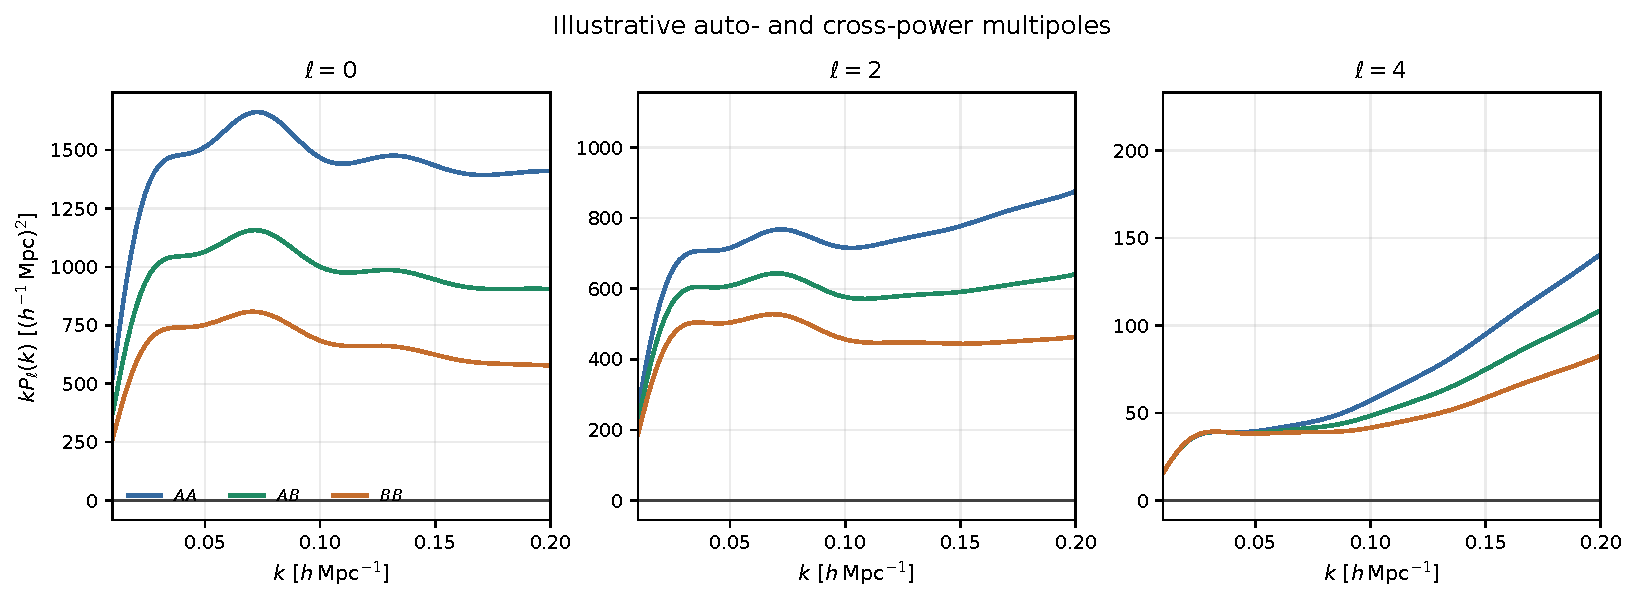
\includegraphics[width=\textwidth]{figures/cross_power_multipoles.pdf}
%   \caption{Illustrative auto- and cross-power multipoles for the LRG-like
%   tracer A, the ELG-like tracer B, and their equal-time cross spectrum. The
%   curves show \(kP_\ell(k)\) for \(\ell=0,2,4\) using the baseline EFT
%   settings and prior-document bias convention.}
%   \label{fig:cross-power-multipoles}
% \end{figure}

% \begin{figure}[t]
%   \centering
%   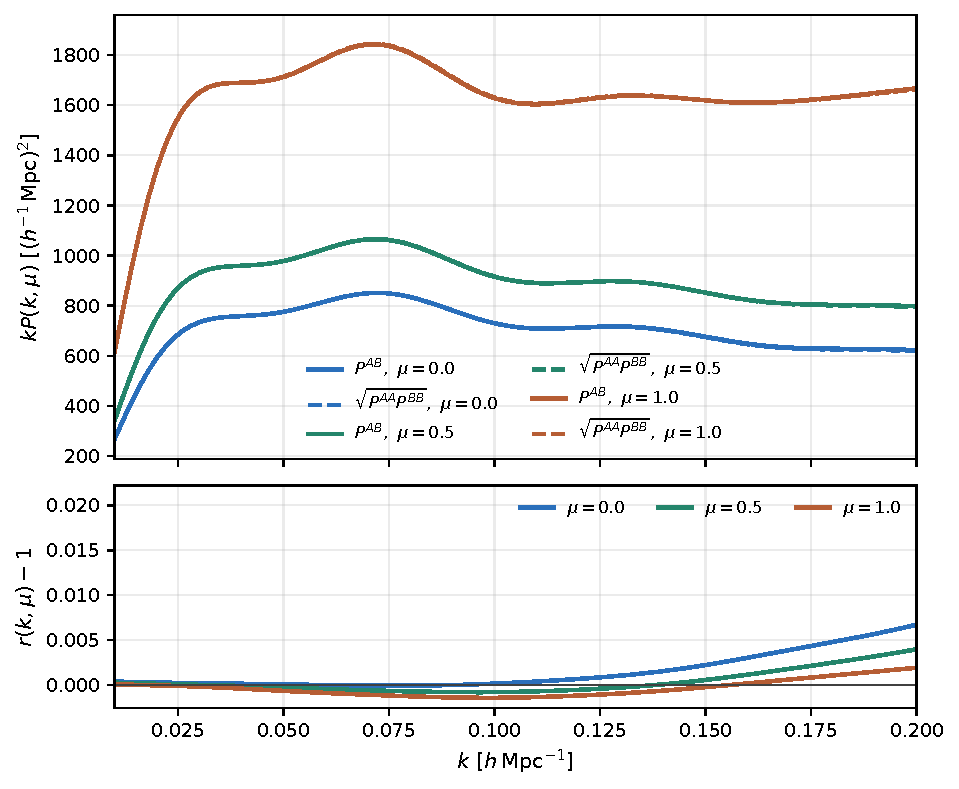
\includegraphics[width=\textwidth]{figures/cross_vs_geometric_mean_pkmu.pdf}
%   \caption{Comparison of the exact implemented \(P^{AB}(k,\mu)\) with the
%   diagnostic geometric mean \(\sqrt{P^{AA}(k,\mu)P^{BB}(k,\mu)}\). The lower
%   panel shows \(r(k,\mu)-1\), where the geometric mean is evaluated only where
%   the square root is real and numerically stable.}
%   \label{fig:cross-vs-geometric-mean-pkmu}
% \end{figure}

% \begin{figure}[t]
%   \centering
%   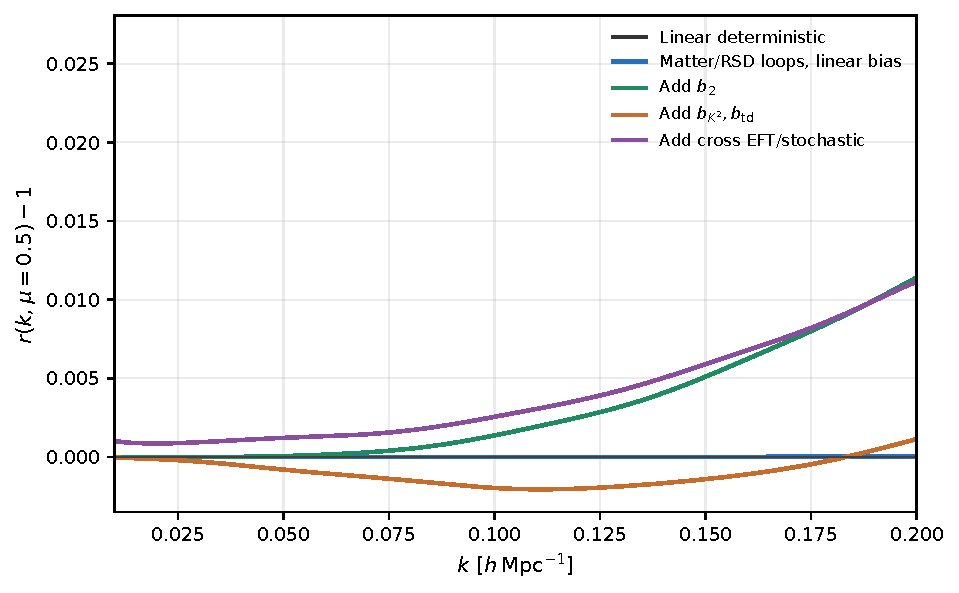
\includegraphics[width=\textwidth]{figures/cross_geometric_mean_bias_dependence.pdf}
%   \caption{Controlled diagnostic for the origin of departures from the
%   geometric-mean approximation. The cases switch on the linear deterministic
%   limit, one-loop matter and redshift-space terms, nonlinear bias terms, and
%   explicit pair-level EFT and stochastic terms.}
%   \label{fig:cross-geometric-mean-bias-dependence}
% \end{figure}

% \begin{figure}[t]
%   \centering
%   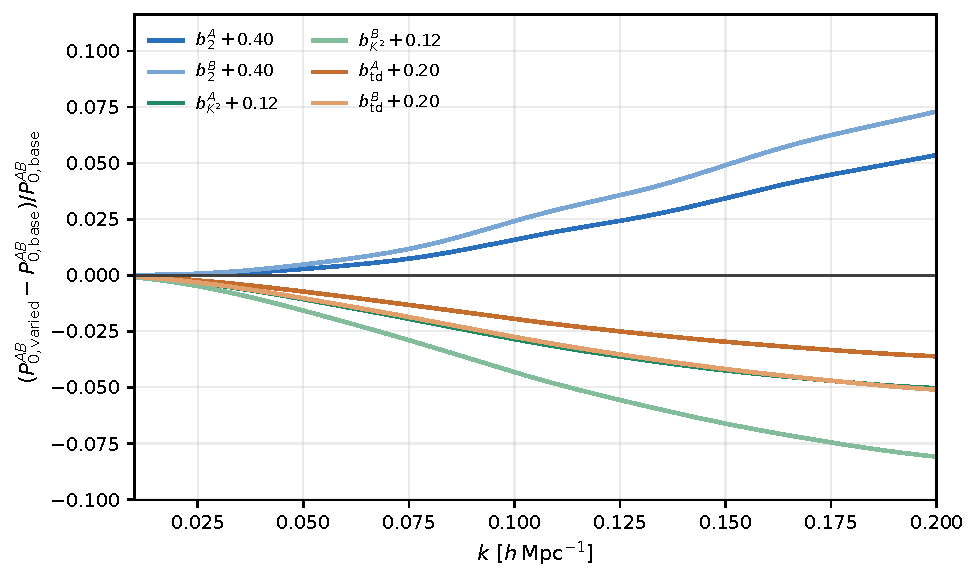
\includegraphics[width=\textwidth]{figures/cross_nonlinear_bias_response.pdf}
%   \caption{Fractional response of the cross monopole \(P_0^{AB}\) when one
%   nonlinear prior-document bias parameter is varied at a time for tracer A or
%   tracer B. The variations are illustrative and are not prior choices.}
%   \label{fig:cross-nonlinear-bias-response}
% \end{figure}

% \begin{figure}[t]
%   \centering
%   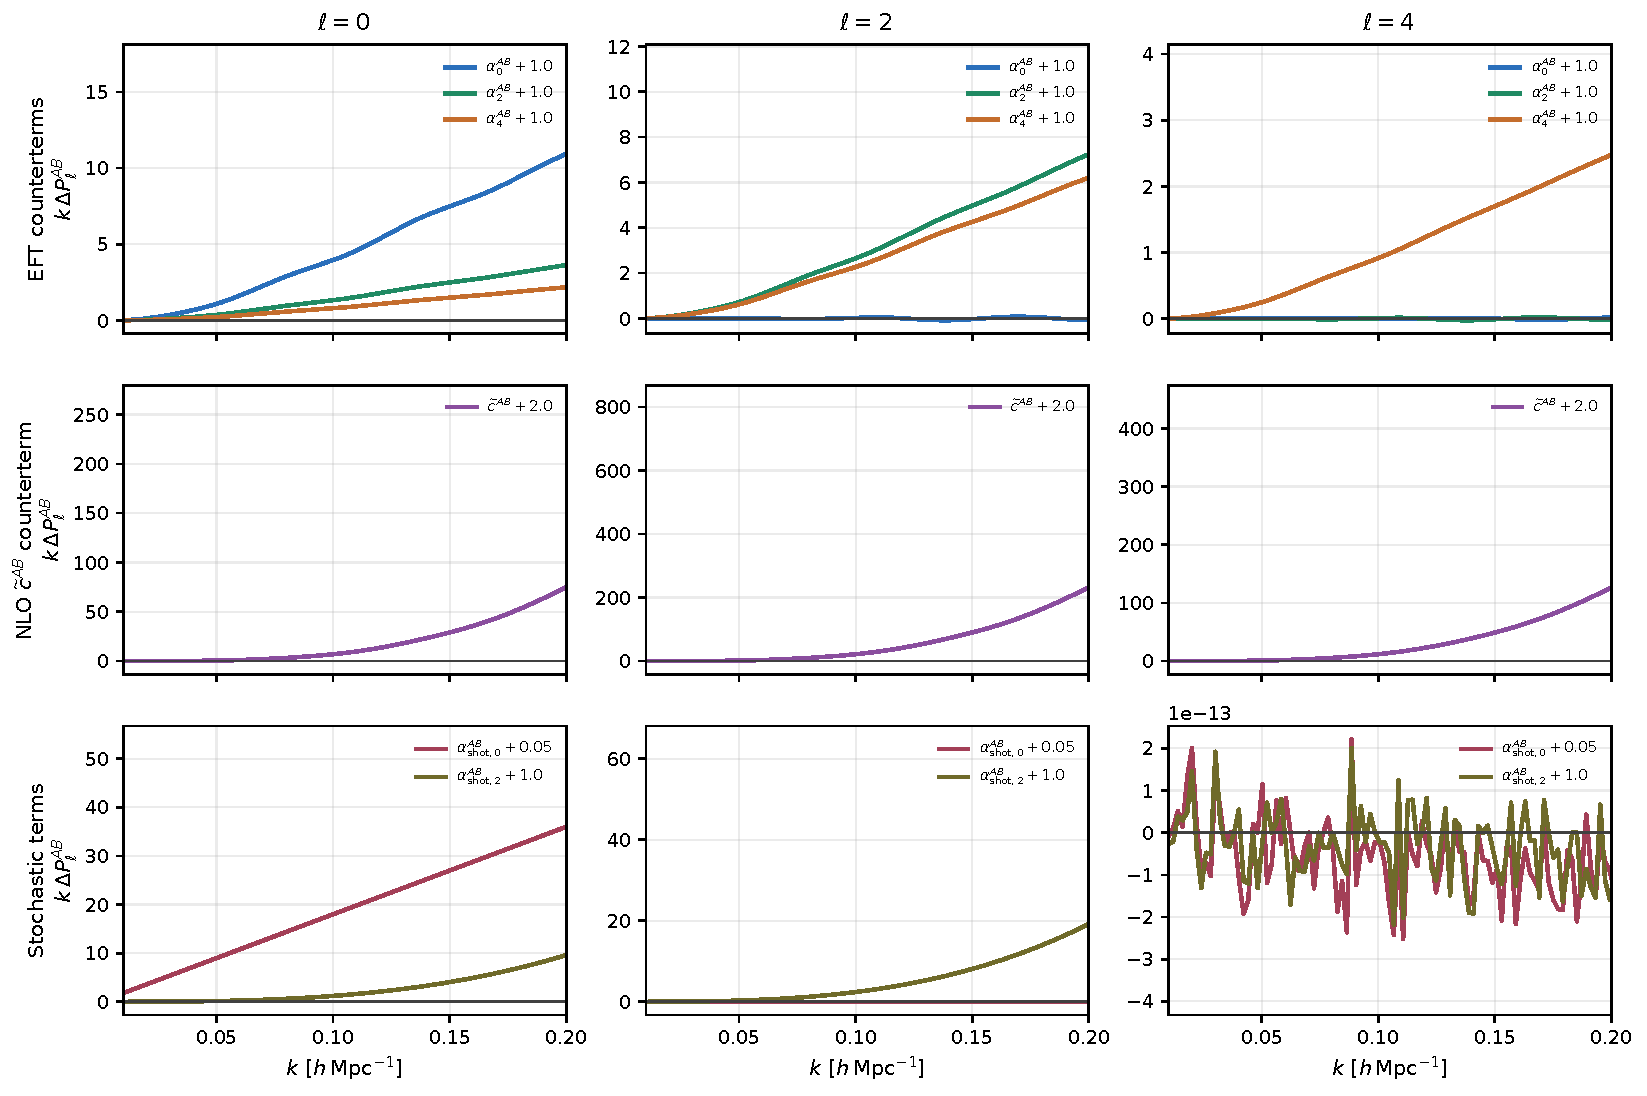
\includegraphics[width=\textwidth]{figures/cross_nuisance_response.pdf}
%   \caption{Response of \(P_\ell^{AB}\) to independent pair-level EFT and
%   stochastic nuisance parameters. The rows isolate the standard EFT
%   counterterms, the NLO \(\widetilde c^{AB}\) counterterm, and the stochastic
%   terms so that smaller responses remain visible.}
%   \label{fig:cross-nuisance-response}
% \end{figure}

% \begin{figure}[t]
%   \centering
%   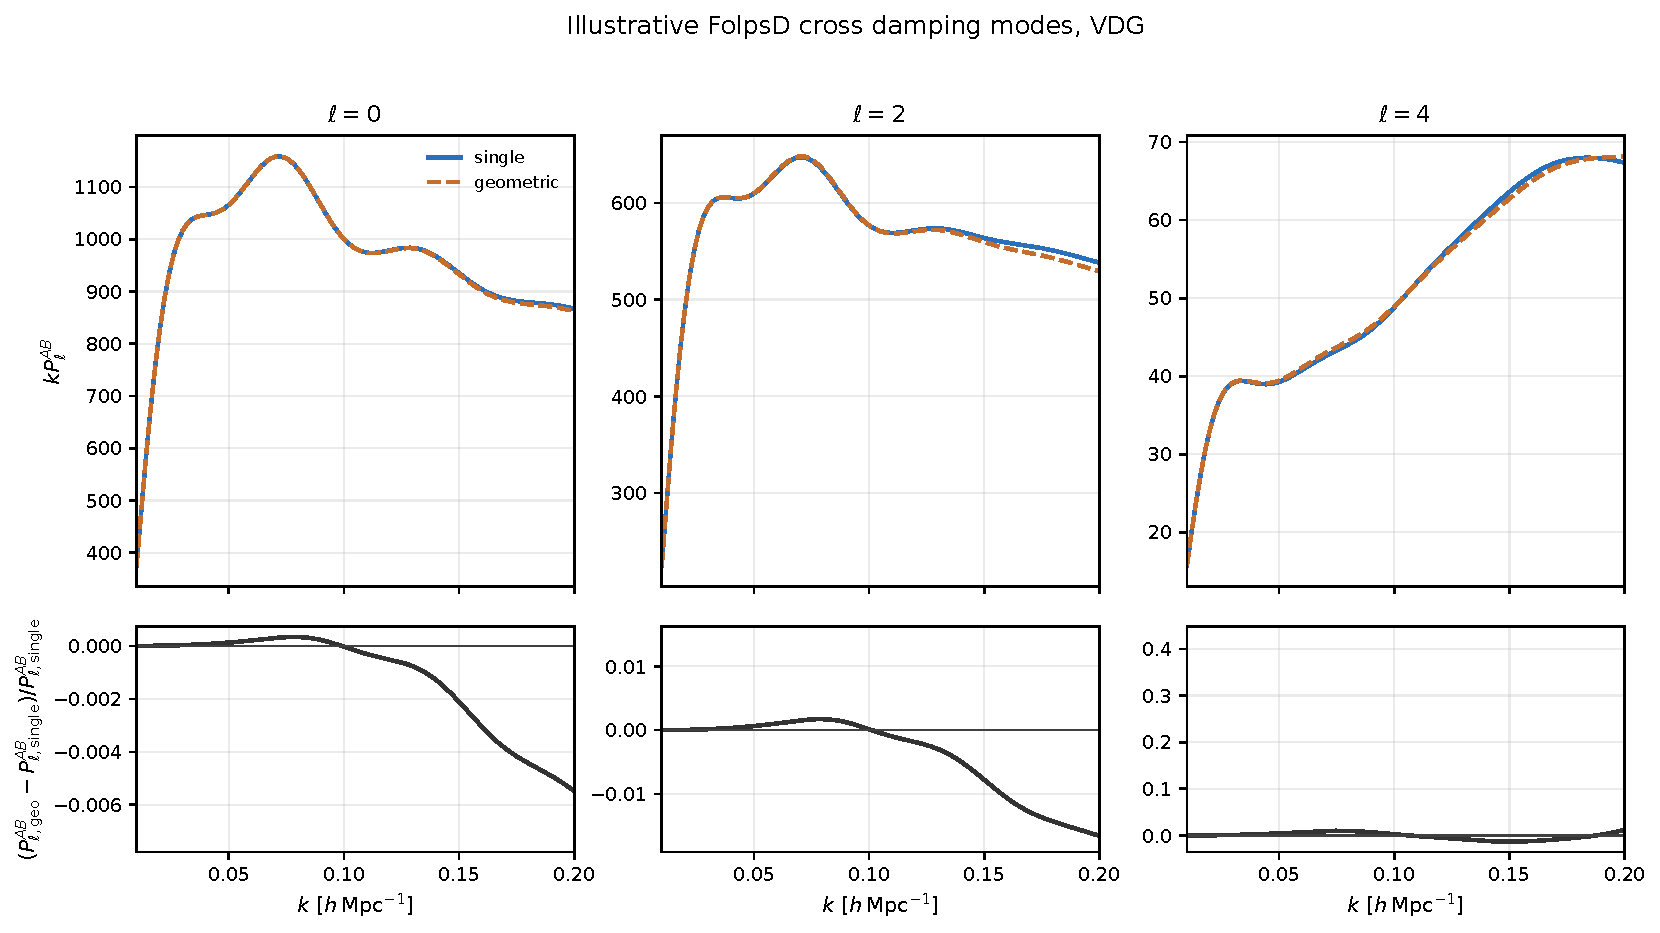
\includegraphics[width=\textwidth]{figures/cross_damping_modes.pdf}
%   \caption{Illustrative FolpsD cross damping comparison for the VDG damping
%   function. The single mode uses one pair-level \(X_{\rm FoG}^{AB}\), while
%   the geometric mode uses \(\sqrt{W(X_{\rm FoG}^{A})W(X_{\rm FoG}^{B})}\)
%   and ignores the pair-level \(X_{\rm FoG}^{AB}\). These are alternative
%   nuisance prescriptions, not first-principles preferences.}
%   \label{fig:cross-damping-modes}
% \end{figure}

% \begin{figure}[t]
%   \centering
%   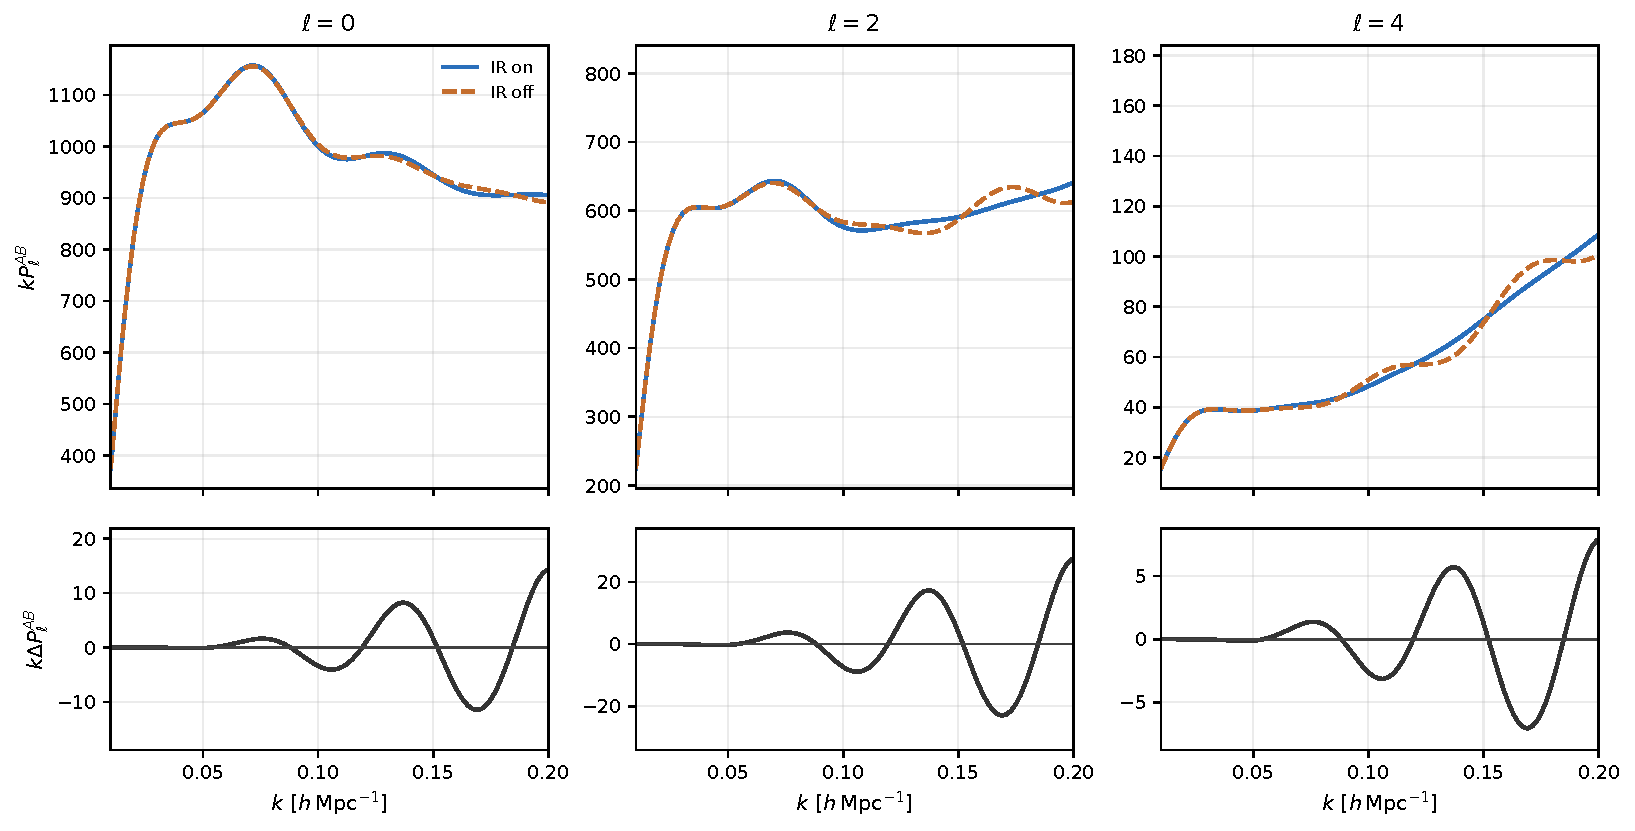
\includegraphics[width=\textwidth]{figures/cross_ir_resummation.pdf}
%   \caption{Numerical effect of IR resummation on the cross multipoles. The
%   upper panels compare the IR-resummed and non-resummed calculations, and the
%   lower panels show the corresponding absolute differences.}
%   \label{fig:cross-ir-resummation}
% \end{figure}

% \begin{figure}[t]
%   \centering
%   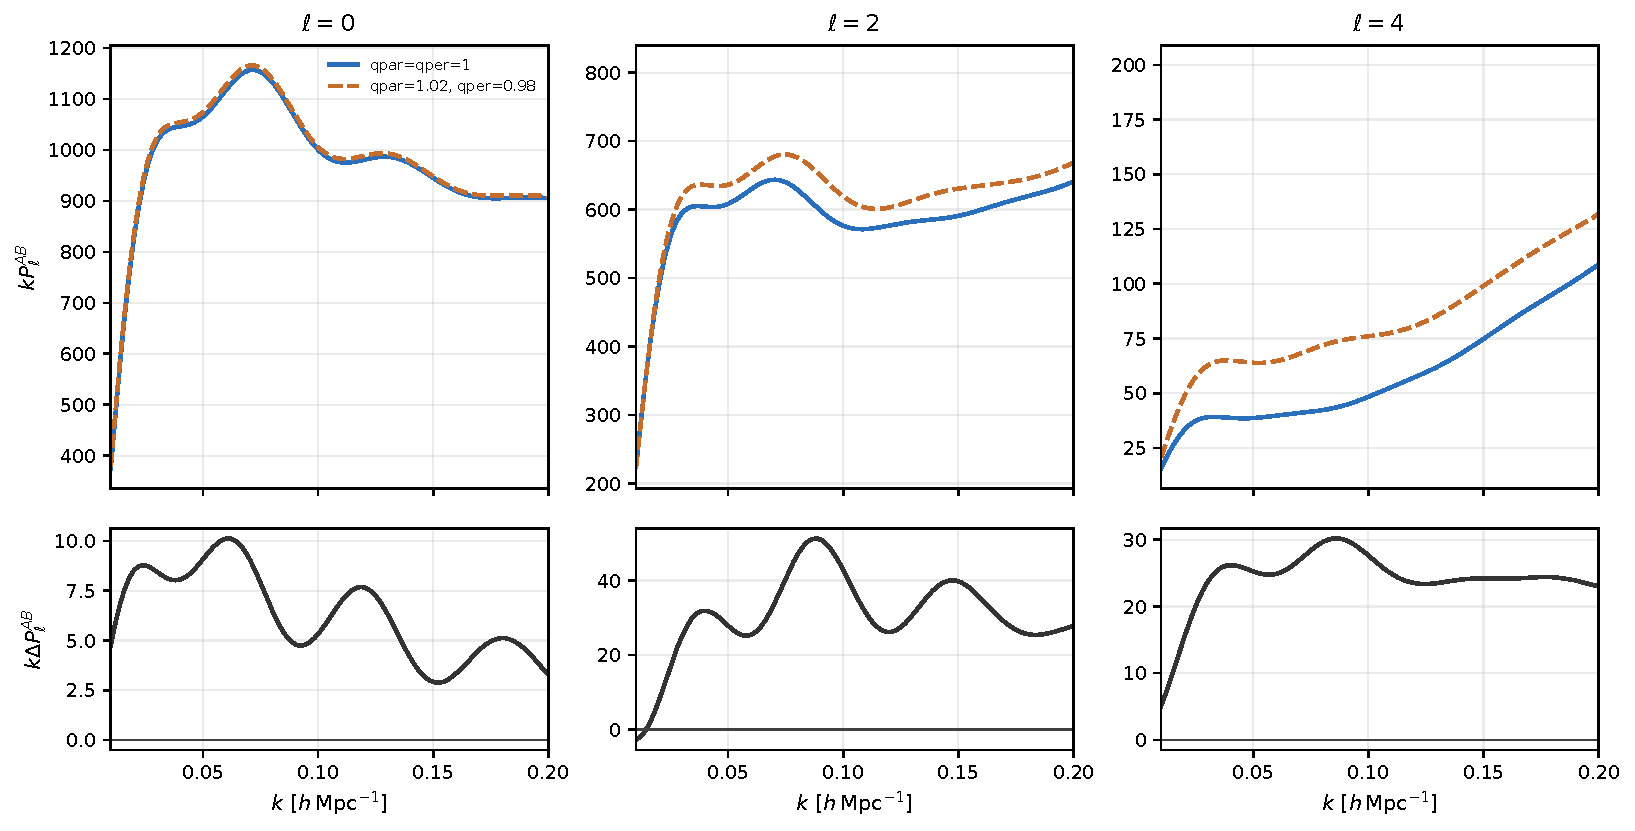
\includegraphics[width=\textwidth]{figures/cross_ap_remapping.pdf}
%   \caption{Illustrative Alcock-Paczynski remapping of the cross multipoles,
%   comparing the fiducial \(q_\parallel=q_\perp=1\) calculation with a small
%   numerical distortion.}
%   \label{fig:cross-ap-remapping}
% \end{figure}

% \begin{figure}[t]
%   \centering
%   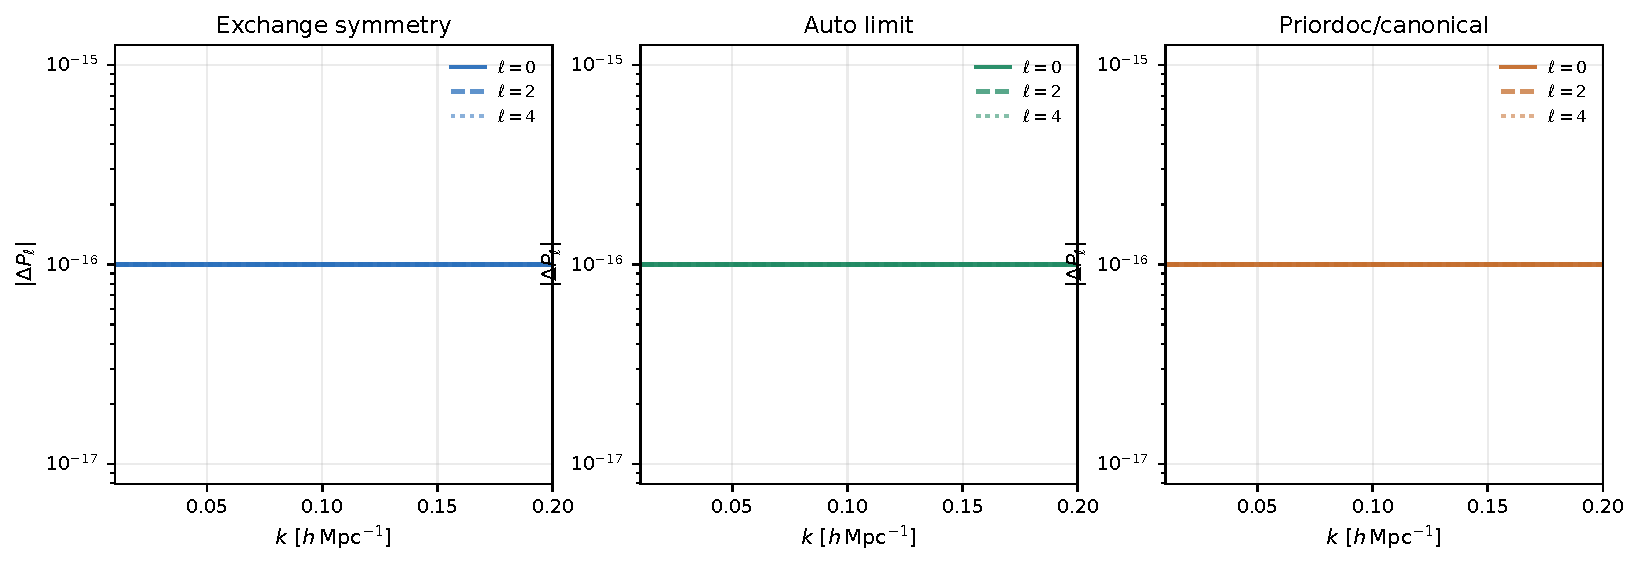
\includegraphics[width=\textwidth]{figures/cross_implementation_residuals.pdf}
%   \caption{Implementation residuals for exchange symmetry, auto-limit
%   recovery, and prior-document versus canonical parameter conversion. The
%   logarithmic plotting floor is used only to display near-zero residuals.}
%   \label{fig:cross-implementation-residuals}
% \end{figure}
